% !Mode\label{key}:: "TeX:UTF-8"
%!TEX program  = xelatex

\documentclass[withoutpreface,bwprint]{cumcmthesis} %去掉封面与编号页
\usepackage[version=4]{mhchem}

\title{2017 CPU iGEM 建模方案 (初稿)}
\tihao{A}

\begin{document}
\setcounter{secnumdepth}{3}
 \maketitle

\section{问题重述} 

\subsection{系统简介}
\begin{figure}[!h]
	\centering
	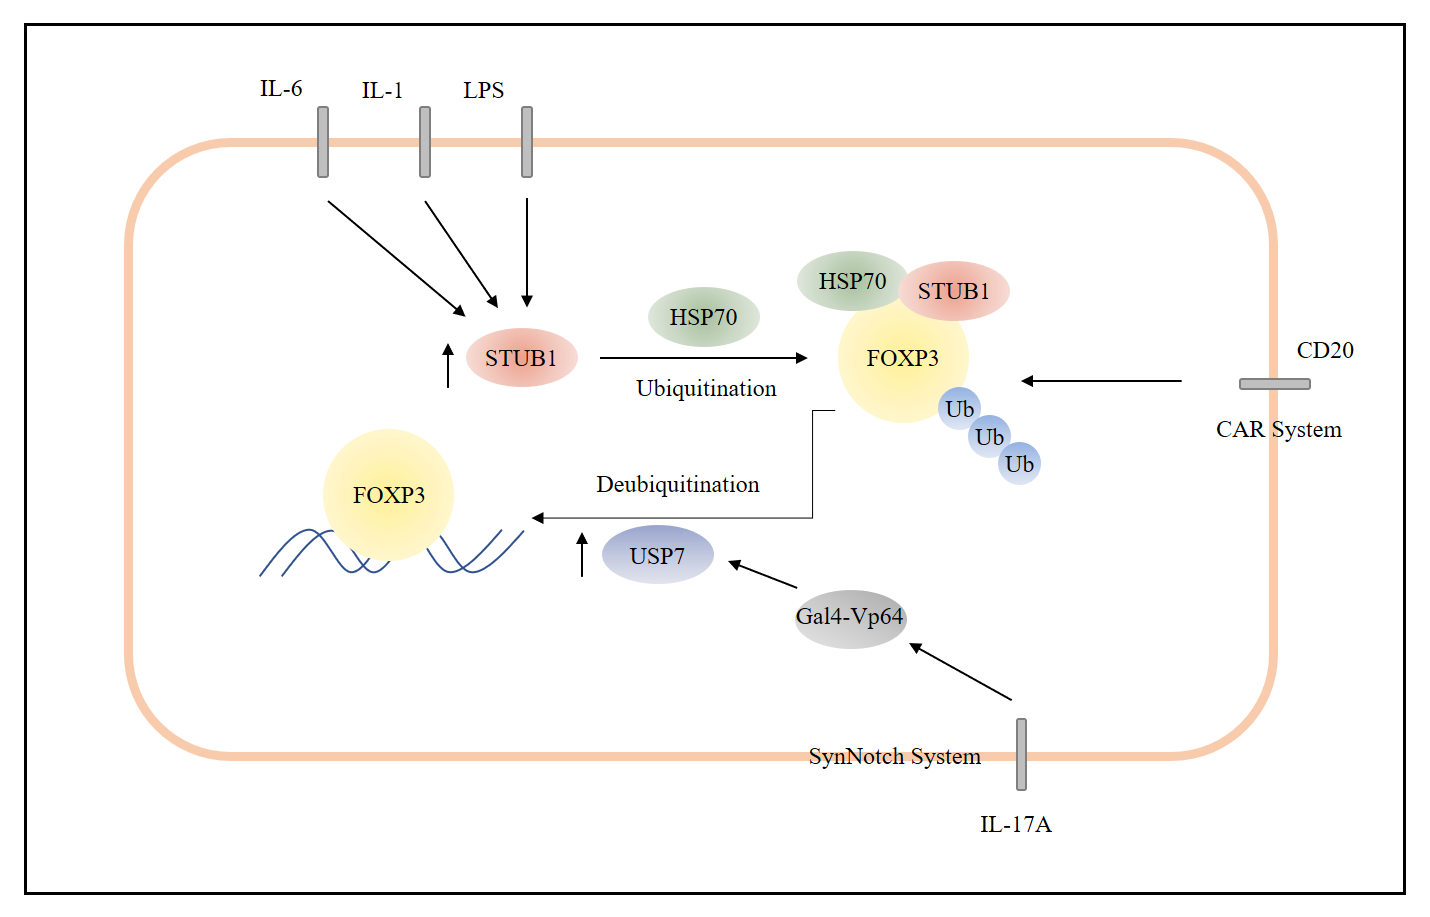
\includegraphics[width=.6\textwidth]{4.png}
	\caption{系统设计示意图}
\end{figure}
如图所示,系统由两部分组成,一部分为构造的Syn-notch系统,另一部分为CAR系统。系统包含的生物学过程有以下几种:

\begin{enumerate}[itemindent=2em]
\item 受体配体相互作用(IL-17A与受体的结合)
\item 受体配体结合后的信号转导动力学(VP64的释放)
\item 基因表达建模:
\begin{itemize}[itemindent=1em]
	\item 启动子识别
	\item 转录的动力学过程
	\item 翻译的动力学过程
\end{itemize}
\item 酶动力学过程:
\begin{itemize}[itemindent=1em]
	\item 蛋白的泛素化-去泛素化过程
\end{itemize}
\end{enumerate}

针对以上所述的生物学过程主要选取基因表达建模与酶动力学过程进行定量分析试图通过实验数据确立相关模型的参数。

\subsection{问题提出}

\begin{enumerate}[itemindent=2em]
\item 通过建立数学模型对生物学系统的一些性质进行预测?例如稳定性,鲁棒性,安全性等。
\item 如何通过数学模型对生物学系统进行优化。
\end{enumerate}
 
\section{问题分析}
针对上述问题需要根据不同的过程逐一进行分析和建模。我们试图寻找一个相对合理但又不失创新性的方案。

\begin{enumerate}[itemindent=2em]
	\item 在项目的开始,我们首先问自己:
	\begin{itemize}[itemindent=1em]
		\item 这样的数学模型要解决什么样的问题?
		\item 这样的数学模型对于这个问题有什么意义?
		\item 这样的数学模型是否足够解决上述问题?
		\item 怎样去建立这样的数学模型?
	\end{itemize}
\end{enumerate}

设计合成生物系统的目的是为了获得目的产物或崭新的生物功能,因此生物模块作为一个功能单元难免被植入到异源或同源生物体中,且必然会受到生物体中诸多信号的影响;合成生物学强调生物模块的“即插即用”性,要保证设计好的生物模块被方便的整合入其他功能模块中,生物模块就必须具有很好的稳定性和抗各种外界干扰的鲁棒性。此外,由于各种蛋白质、激酶自身的降解,为了维持宿主细胞内环境中各种蛋白质、代谢产物的平衡,生物模块必须具有很好的快速响应特性,能够以足够快的速度接收输入信号做出反应。
因此,分析生物模块的稳定性、鲁棒性和快速响应特性等属性,总结和抽提设计的普遍原则,对于生物模块的功能扩展和生物系统的工程化至关重要。
我们针对上述生物学过程逐一分析。
\subsection{受体配体相互作用(IL-17A与受体的结合)}
\begin{figure}[!h]
	\centering
	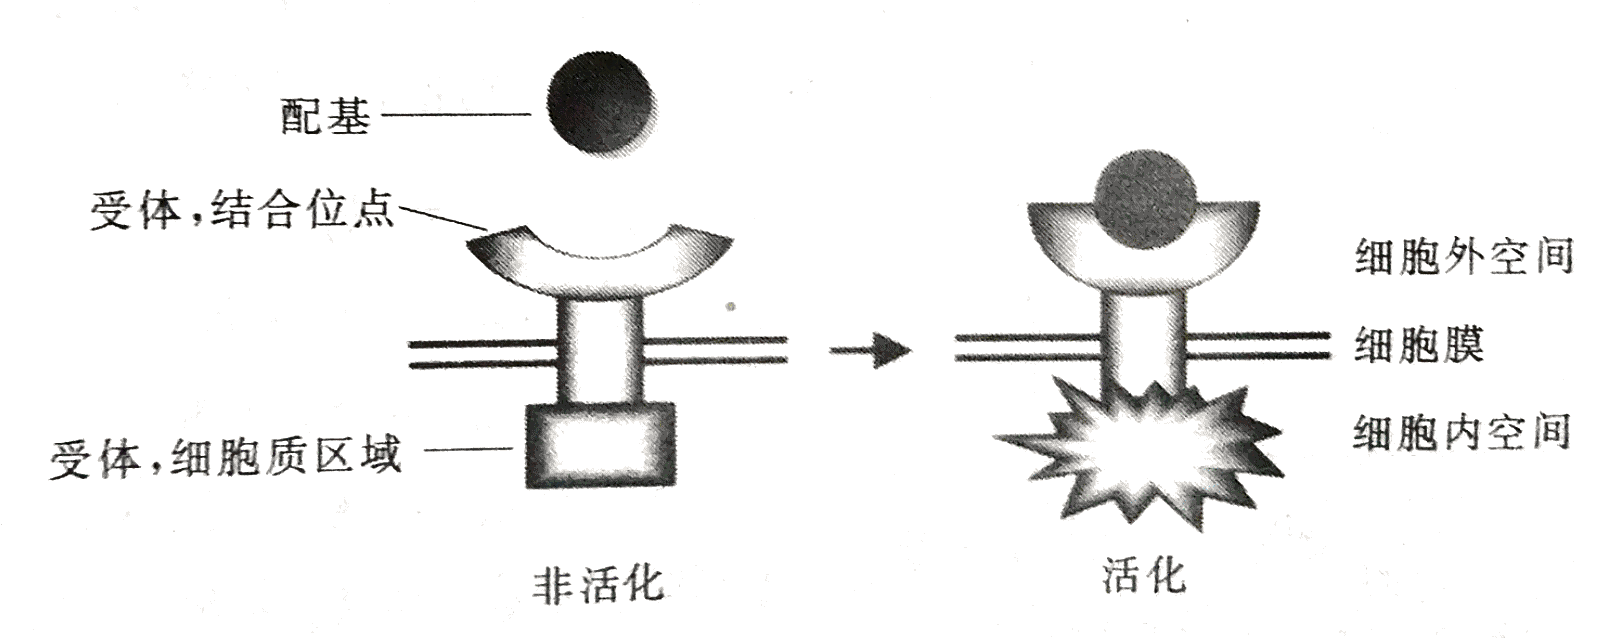
\includegraphics[width=.6\textwidth]{1.png}
	\caption{受体和配体结合示意图}
\end{figure}

针对syn-notch蛋白在受到信号刺激后与其相连的Gal-VP64 脱落这一过程可以抽象成一组微分方程(ODE)。
$$\frac{dR}{dt} = f(S,r)$$   
这里S为信号强度(例如IL-17A 浓度,R等于输出信号强度(VP64浓度,r为受体浓度)。

对于这样一个ODE系统建模时我们最关心的问题就是参数的选取问题,关于这一问题可以尝试先从文献或数据库中查询相关数据再参考2016年曼彻斯特大学数学建模部分所使用的方法:
基于参数检验和非参数检验的参数拟合方法。

\subsection{基因表达建模}
基因表达建模是科学领域中通过不同的技术获得结果的一个例子。基因表达的结果和动力学通过布尔网络、贝叶斯网络、有向图、常微分方程与偏微分方程系统、随机方程和基于规则的形式方法等手段进行了数学上的描述。
\begin{itemize}
\item 启动子识别:
\end{itemize}

针对我们设计的启动子查询相关的生物信息学数据库,主要包括启动子强度以及转录因子与启动子序列结合的相关参数。

\begin{itemize}
\item 转录和翻译的动力学过程:
\end{itemize}
	
转录和翻译的动力学过程类似之前提到的受体配体相互作用模型,同样适用ODE系统进行描述,只是方程形式稍有区别。查阅相关书籍和文献后可知真核基因表达特定过程的建模可以使用多种方法,但针对定量模型ODE系统具有不可替代的优势,因而较多的被使用。

ODE系统中的参数确定问题(主要以米氏动力学为主)同样也是较为困难的,通常以查阅文献和数据库的方式,但经过分析后发现使用数据挖掘方法辅助确定参数比较合理与准确(参见具体建模过程)。

\subsection{蛋白的泛素化与去泛素化过程}

\begin{center}
	\ce{Ub-FoxP3 <=>[{USP7}][{Stub1}] FoxP3}
\end{center}

此部分主要建立不同机理下的酶促反应动力学模型。可尝试使用数据对机理进行探究或通过实验数据拟合动力学参数。

与上述模型类似,蛋白的去泛素化过程同样可表示成一系列基于希尔函数的ODE系统。稍有不同的是,根据反应的机理,其方程形式不同。上述反应中所涉及的两个酶(USP7与STUB1)的动力学参数可以从BRENDA数据库中获取。

考虑对整个模型的建模,整个模型可看作黑箱模型,不考虑其内部结构,仅注意到它对于信息刺激作出的反应,注意它的输入-输出关系,以此确定黑箱中的参数与函数形式。


鉴于自体Treg细胞分离培养十分困难,另外,动物实验与B细胞共培养实验也难以进行,更为重要的是,实验使用的Jurkat细胞系十分特殊,对于上述问题的建模也十分局限。因此,建模必须在几乎不依靠实验数据的基础上来进行,从合成生物学角度来讲,对于合成生物系统的建模中,通用的方法是工程化的,一般分析合成生物系统的性能,主要有以下几个主要指标:
\begin{itemize}[itemindent=1em]
	\item 稳定性
	\item 鲁棒性
	\item 响应快速性
\end{itemize}

其中稳定性和鲁棒性(又称稳健性)较为重要,我们将着重选取其中的稳定性指标进行重点分析。

系统的稳定性对于我们的系统是十分重要的,因为我们的系统是用于治疗的一种尝试,首先考虑的应该是安全性的问题,通过实验测定黑箱系统的工作参数,以此设定治疗方案或优化系统设计,这对该项目设想将来的发展具有重要的参考价值。

在考虑了系统的安全性后,下一个重要指标也就必须列入考虑范围内:有效性,有效性和安全性对于一个系统而言就如数学证明中充分性与必要性一样,一个治疗系统在保证安全性的条件下,首先要考虑的应该是有效性,有效性的评价方法是多样的,一般可通过与对照组的实验得出,在这种情况下,对照组通常是有效性得到确定评价的,但由于我们项目的特殊性,这一方法难以实行。这里,我们考虑单纯从验证系统中各组件运行状态出发,先通过模拟建模,再以实验数据进行模型的修正,计算系统在各参数下运行的状态。




\section{模型建立}
\subsection{基于机器学习的实验数据挖掘与参数计算}
\subsubsection{机器学习概要}
Machine Learning(机器学习)是研究计算机怎样模拟或实现人类的学习行为,以获取新的知识或技能,重新组织已有的知识结构使之不断改善自身的性能。
目前存在几种不同类型的学习算法。主要的两种类型被我们称之为监督学习和无监督学习。下面介绍我们采用的具体机器学习方法。

\begin{tabbing}
无监督学习:
\end{tabbing}

无监督学习最重要的用途应该就是用来研究分类问题,通过对数据进行聚类分析,主成分分析,最终找出数据中的关键因素,以及找出数据之间潜在的类别。这些在经典的统计学中是很难做到的,但是借助现代计算机的高速运算能力,我们可以让计算机通过对数据进行“学习”,从而对数据进行分类。
\begin{figure}[!h]
	\centering
	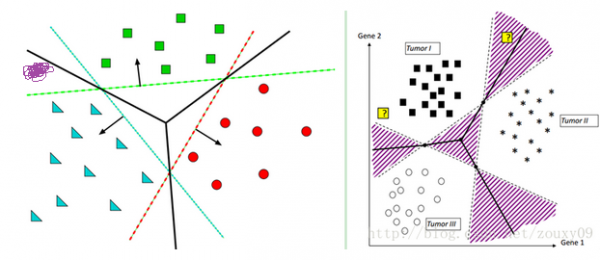
\includegraphics[width=.6\textwidth]{2.jpg}
	\caption{无监督学习二维空间分类示意图}
\end{figure}

\begin{tabbing}
异常值检测:
\end{tabbing}

异常值检测是基于多元高斯分布的一种机器学习算法,它可以允许我们使用训练集对模型进行训练,并通过交叉测试集对模型进行改进提高预测的准确性,降低误报率,最终可以利用测试集对模型进行评估,从而实现对系统的安全性和稳定性进行评估。
\begin{figure}[!h]
	\centering
	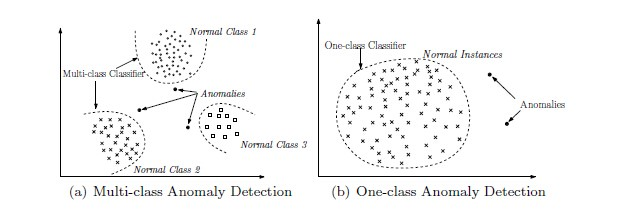
\includegraphics[width=.6\textwidth]{3.jpg}
	\caption{异常值检测示意图}
\end{figure}

\subsubsection{如何用此方法进行数据挖掘和参数计算}
\begin{enumerate}[itemindent=2em]
	\item 利用无监督学习找到系统潜在的稳态\\
	 \qquad 对于这样一个复杂体系,难免会出现很多稳态,但是发现这些稳态是比较困难的,因此可以使用机器学习中的无监督学习对系统的稳态进行挖掘。通过聚类分析,可以讲数据点聚成多维空间中的一些类,这些类很可能就是一些潜在的系统稳态,因为如果数据能够成簇出现,那么这个类中心所对应的动力学参数大多是稳定的(可以用微分方程的向量场理论解释)。因此用非监督学习对数据分类可以指导后期进行动力学建模。
	\item 利用异常值检测方法评估系统的稳定性\\
	 \qquad 异常值检测方法实际在医学中应用广泛,比如我们用一些疾病的患者和正常人血常规的数据训练对模型进行训练,然后有病人的新的数据输入后,模型可以指示此病人的血常规是否正常以及可能患有什么疾病。实际医生看病的原理和这个差不多,只是我们这里不是训练一个医生,而是训练一个机器。
	我们通过异常值检测模型,可以预测我们的系统是否工作正常,以及如果不正常是出了哪方面的问题。
\end{enumerate}
\subsubsection{所需的实验数据}
在不同IL-17A浓度梯度和时间梯度下的Foxp3,USP7。以及Foxp3,USP7的mRNA的QPCR数据(非必须)

\begin{table}[htb]
	\centering
	\caption{实验数据采集示意表}\label{tab:one}
	\begin{tabular}{|c|c|c|c|}
		\hline
		     & C1 & C2 & Cn \\ \hline
		  t1 &    &    &    \\ \hline
		  t2 &    &    &    \\ \hline
		  tn &    &    &    \\ \hline
		\end{tabular}
	\end{table}
\subsubsection{对于方案存在的问题进行讨论(模型优缺点),可行性等}
\begin{tabbing}
优点:
\end{tabbing}

对于这样的一个模型,我们的优点是模型的算法较为先进,由于这是一个生物复杂系统,我们很难像测量一个机械系统那样做到数据量大准确。我们能测量的数据很少,并且每个数据的测量代价都非常大。因此在这种情况下经典统计学的方法都失效了,因此我们通过建模的分析想找到一种可以用少量数据就可以达到较好的效果的方法,因此决定采用机器学习的方法,机器学习在处理复杂系统方面非常有优势,因为它的算法非常类似人类的思考方式。

\begin{tabbing}
	缺点:
\end{tabbing}

当然,再好的算法如果没有数据也是不行的,所以缺点是我们的数据可测量难度大,数据量小。因此我们再保证能够完成的情况下尽可能多的数据点,这样模型会更加精确。

\begin{tabbing}
	可行性:
\end{tabbing}
	
我们数模组成员之前都学习过一些机器学习的知识,也做过一些真实的案例。实验方面量也不是很大,在保证完成主要实验的基础上可以完成,当然这些实验数据对于我们的课题也是非常有必要的。


\subsection{外部噪声诱导的状态切换}
\subsubsection{噪声与细胞状态的切换}
在有外部噪声干扰时,反应速率本身是随机变化的,使用化学反应主方程来描述系统的行为并不合适。这是因为此时对系统的状态空间的完备描述除了需要指导系统中各种分子的个数,还需要指导反应速率的状态,而这是不可能的。因此,我们使用推广的化学郎之万方程来同时描述系统的内部噪声和外部噪声。
$$dX_1=(\lambda_{1+}(n-X_1)-\lambda_1 X_1)dt+\sqrt{\lambda_{1+}(n-X_1)}dW_1-\sqrt{\lambda_{1-}X_1}dW_2$$
$$dX_2 = (\lambda_2X_1-\delta_2X_2)dt+\sqrt{\lambda_2X_1}dW_3-\sqrt{\delta_2 X_2}dW_4$$
$$dX_3=(\lambda_3X_2-\delta_3X_3)dt+\sqrt{\lambda_3X_2}dW_5-\sqrt{\delta_3X_3}dW_6$$

中$W_i(i=1,2,...,6)$为相互独立的维纳过程。	
下面考虑存在外部噪声的情况,如果在上面的化学郎之万方程中的某个参数,例如$\lambda_{1+}$是随机变化的,可以用下面满足对数正态分布的随机过程来描述:

$$\lambda_{1+}(t)=\lambda_{1+}\frac{e^{f_{\lambda_{1+}}\eta_{\lambda_{1+}}(t)/\lambda_{1+}}}{<e^{f_{\lambda_{1+}}\eta_{\lambda_{1+}}(t)/\lambda_{1+}}>}$$

在这里为了避免符号的繁琐,还以$\lambda_-$和$\lambda_+(t)$的统计平均,并设为常数。这里$f>0$为常数,表示外部噪声的强度,$\eta_+$为标准白噪声。
\subsubsection{外部噪声对基因表达的影响}
根据上面的结果,来分析外部噪声对基因表达的随机性影响。
首先来看只有外部噪声的情况。将的外部扰动项设为零,则可以得到只有外部噪声时系统的静态涨落。

$${\eta_{ext,1}}^2 = k_1 \frac{\lambda_{1-,obs}}{\delta_{1-,obs}}\frac{1}{2}(\frac{\xi_{\lambda_{1+}}}{g_1})$$

$${\eta_{ext,2}}^2 = k_2[\frac{1}{2}(\frac{\eta_{\lambda_2}}{g_2}(1+{\eta_{ext,2}}^2)+\xi_{\delta_2})+\frac{\tau_1}{\tau_1+\tau_2}{\eta_{ext,2}}^2]$$

$${\eta_{ext,3}}^2 = k_3[\frac{1}{2}(\frac{\eta_{\lambda_3}}{g_3}(1+{\eta_{ext,2}}^2)\xi_{\delta_3})+\frac{\tau_1\tau_3/\tau_2}{\tau_1+\tau_3}\frac{\tau_1}{\tau_1+\tau_2}\frac{\tau_2}{\tau_2+\tau_3}{\eta_{ext,1}}^2+\frac{\tau_2}{\tau_2+\tau_3}{\eta_{ext,2}}^2]$$

由式上式可知,和内蕴随机性类似,外部噪声对静态涨落的影响也可以区分为直接的涨落和因为上游分子数的涨落所引起的间接涨落.例如在蛋白质分子数量的涨落公式中,除了与$\eta$和$\xi$成正比的直接涨落项外,还包含因为上游的激活基因数的随机性和mRNA分子数的随机性引起的间接涨落项,分别与$\eta_1$和$\eta_2$成正比.并且,这些间接涨落项都与转录和翻译时间因子有关。另外,mRNA分子数的随机涨落和翻译效 率波动之间的相关也会增加蛋白质数童的涨落,通过项$\frac{1}{2} \frac{\xi}{g_3}$给出.最后,与内蕴随机性最重要的区别是这些静态涨落都正比于影响因子$k$,当噪声强度$\xi$比较大时(接近2),影响因子可以变得很大,也即基因表达水平的涨落非常显著。这一结果表明在基因调 控中,为了控制基因表达的随机性,控制mRNA和蛋白质分子的分解速率的随机性是非常重要的。

状态切换是基因调控的一种常见现象,表现为细胞的状态可以从一种稳定状态很快地 变换到另外一种稳定状态.这种现象对很多生命体,特别是低等单细胞生命,为适应环境变 化而迅速做出响应是特别重要的。对于有正反馈和协作的基因调控网络,系统可 以表现出双稳态。然而,这样还不能实现让系统在两种状态之间切换.要实现状态的切换,还 需要一种机制使得稳定的状态失稳.随机噪声通常是这种失稳的原因。

\subsection{稳定性分析与鲁棒性分析}
\subsubsection{稳定性分析}
目前对于系统的稳定性分析还是主要建立在系统模型的基础之上,对于模型的精度具有一定的依赖性。一般可以采用两种方法来分析其稳定性:解析法和数值法。解析法分析通常需要繁琐的运算,对于没有解析解的模型来说甚至根本行不通,因此通常采用数值解法来分析系统的稳定性。

相位面分析是数值分析的常用方法。通过绘制模型解的近似曲线,相位面分析能够判断系统的稳定性。在相位面分析中通常用模型的雅可比矩阵(Jacobian matrix)来分析稳定性。在向量微积分中,雅可比矩阵是一阶偏导数以一定方式排列成的矩阵,其行列式称为雅可比行列式。雅可比矩阵的重要性在于它体现了一个可微方程与给定点的最优线性逼近。因此,雅可比矩阵类似于多元函数的导数。通过雅可比矩阵的特征值可以判断系统的稳定性。通常正实数特征值说明系统不稳定,负实数特征值说明系统稳定,虚特征值说明系统处于临界状态。
因为微分是系统中偏导数的线性变换,因此方程中每一个线性独立的部分可以看成是特征函数M0,满足约束条件其中,A为特征值。负的特征值代表的特性分量会随着时间而衰减,属于稳态分量。正特征值代表的特性分量则会随着时间的增加而发散,属于不稳定分量。虚根代表的特性分量处于临界状态,需根据具体问题进行具体分析。
\subsubsection{鲁棒性分析}
鲁棒性分析关心的是系统参数发生摄动时,系统能否保持原有的性能和状态,因此需要分析参数变动对于状态的影响,即参数敏感性分析。敏感性分析并不能得出真实的速率常数,只是辅助确定哪个参数更重要。在知识不完备情况下进行系统设计时,确定对系统输出具有最显著影响的参数是至关重要的:如果需要维持系统性能,则应尽量维持最敏感的参数不变;如果需要改变系统性能,则改变最敏感参数可能是最便捷的途径,因为系统输出通常只对少数几个参数敏感,相应突变的候选反应数量则完全可能缩小到实验可以处理的范围内。\\
参数状态敏感性是相对于单独的参数扰动的状态稳定性而言的,以$x(t)$为状态向量,$\rho$为时变参数向量,$f(x(t),\rho)$为具有导数$F(x(t),\rho)$的系统动态矩阵$S_{ij}$代表状态$i$对参数$j$的敏感性,有
$$S_{ij}=\frac{dx_i(t)}{d\rho_j}$$
根据链式法则可以得出所有状态的参数敏感性:
$$\frac{(t)}{d\rho}=\frac{\partial F(x(t),\rho)}{\partial x} S(t)+\frac{\partial F(x(t),\rho)}{\partial \rho}$$
其中,$S(t)$代表特定时间$t$所有的状态敏感性(status sentitivity)。由此可以衡量时间周期$\tau$内的敏感性,作为震荡频率或者周期的无偏估计。从Shape Sensitivity 度量$S(t) = (\frac{\delta x(t)}{\delta \rho})_\tau$的定义可以看出,状态名感性$S(t)$可以看作是Shape Sensitivity和Period Sensitivity 的组合:
$$S(t) = S(t)-\frac{t}{\tau}F(x(t),\rho)\frac{d\tau}{d\rho}$$
其中,Shape Sensitivity 独立于Period Sensitivity。利用仿真工具即可获得微弱的扰动对系统特定部分的影响。\\
敏感性变化独立于影响类型(震荡、稳态或混沌)。参数与真是系统具有直接联系,他们的敏感性能够按时他们所代表的物理对应物的重要性。一般可将参数分为四大类:转录和翻译控制参数、mRNA和蛋白质的降解参数、转运反应参数、蛋白磷酸化和去磷酸化参数。同一类参数的敏感性具有一定的相似性。\\
为了全面衡量系统的鲁棒性,必须同时考虑单参数和多参数的摄动。通常复杂系统中,单个参数的摄动会被其他分支减弱,因此复杂系统对于单参数的摄动有更高的鲁棒性。而多参数系统复杂性的变化会比单回路模型更易导致周期的偏离。
\section{参考文献}





\end{document}



